We present some examples that illustrates the use of Qlang in solving quantum computing problems.

\subsection { Solving Quantum Computation Problem}
\subsubsection{Problem1}
Evaluate the following expressions: a. $(H \otimes X) \ket{00}$ b. $\dotproduct[101,000]$ c. $\bra{01} H \otimes H \ket{01} $
\begin{lstlisting}
	
def compute() : mat evaluate (){
	mat a;
	a = |00>;
	evaluate = (H @ X) * a;	
	printq(evaluate);
				
}
	
\end{lstlisting}

\subsubsection{Problem 2}
Consider the circuit and show the probabilities of outcome 0 where $\ket{\Psi_{in}} = \ket{1}$
\begin{figure}[h!]
\begin{center}
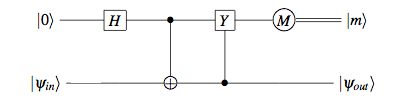
\includegraphics{ref/circuit2}
\end{center}
\caption{ Quantum Circuit\label{cir1}}
\end{figure}

\begin{lstlisting}
def measure(mat top): mat outcome{
        mat ad;
        
        ad = adj(top);
        outcome = top*ad;
}

def outcomezero(mat bottom) : float probability{
        
        mat top; mat input;
        mat had; mat cnot; mat ynot;
        mat output;  mat meas;
        
        top = |0>;
        input = top @ bottom;
        
        had = H @ IDT;
        cnot = [(1,0,0,0)
                (0,1,0,0)
                (0,0,0,1)
                (0,0,1,0)];
      
        
        ynot = [(1,0,0,0)
                (0,0,0,-1)
                (0,0,1,0)
                (0,-1,0,0)];
    
        output = (ynot*(cnot*(had*input)));
        
        printq(output);
        
        probability = norm(output);
   
}

def compute() : float outcome{
        
        mat bottom;
        
        bottom = |1>;
        outcome = outcomezero(bottom);
        print(outcome);
	
}
\end{lstlisting}

\subsection{ Simulation of Quantum Algorithm}

\subsubsection{Deutsch Jozsa Algorithm}
\begin{lstlisting}
def measure (mat top) : mat outcome{
        
        mat ad;

        ad = adj(top);
        outcome = top * ad;
}

def hadamard (int n) : mat gate{
        
        int i;
        gate = H;

        for (i from 0 to n-1 by 1){
            gate = gate @ H; 
        }
}

def topqubit (int n) : mat input{

        int i;
        input = |0>;

        for (i from 0 to n-1 by 1){
                input = input @ |0>;
        }          
}

def deutsch (int n, mat U) : float outcomeZero{

        mat bottom; mat top; mat input;
        mat hadtop; mat meas;

        bottom = |1>;
        top = topqubit(n);
        input = top @ bottom;
        
        hadtop = hadamard(n);
        input = (hadtop @ H)*input;
        input = U * input;
        input = (hadtop @ IDT)*input;
        meas = measure(top);

        input = (meas @ IDT)* input;
        outcomeZero = norm(input);
}


def compute () : float outcome{

        int n; mat Ub; mat Uc;

        n = 1;
        Ub = [(1,0,0,0)(0,1,0,0)(0,0,0,1)(0,0,1,0)];
        Uc = [(1,0,0,0)(0,1,0,0)(0,0,1,0)(0,0,0,1)];

        outcome = deutsch(n, Ub);
        print(outcome);
        
        outcome = deutsch(n, Uc);
        print(outcome);

        n = 2;
        Ub = [(1,0,0,0,0,0,0,0) 
              (0,1,0,0,0,0,0,0)
              (0,0,1,0,0,0,0,0)
              (0,0,0,1,0,0,0,0) 
              (0,0,0,0,0,1,0,0) 
              (0,0,0,0,1,0,0,0)
              (0,0,0,0,0,0,0,1)
              (0,0,0,0,0,0,1,0)];

        outcome = deutsch(n, Ub);
}

\end{lstlisting}

